\documentclass[a4paper]{article}

\input{style/ch_xelatex.tex}
\input{style/scala.tex}

\lstset{numbers=left,
basicstyle=\tiny,
numberstyle=\tiny,
keywordstyle=\color{blue!70},
commentstyle=\color{red!50!green!50!blue!50},
frame=single, rulesepcolor=\color{red!20!green!20!blue!20},
escapeinside=\`\`
}

\graphicspath{{fig/}{fig/generated/}}
\usepackage[fontset=none]{ctex}
\usepackage{graphicx}
\usepackage{color,framed}
\usepackage{listings}
\usepackage{caption}
\usepackage{amssymb}
\usepackage{enumerate}
\usepackage{xcolor}
\usepackage{bm}
\usepackage{lastpage}
\usepackage{fancyhdr}
\usepackage{tabularx}
\usepackage{geometry}
\usepackage{graphics}
\usepackage{subfigure}
\usepackage{float}
\usepackage{pdfpages}
\usepackage{pgfplots}
\pgfplotsset{width=10cm,compat=1.9}
\usepackage{multirow}
\usepackage{footnote}
\usepackage{booktabs}
\usepackage{hyperref}

\setCJKmainfont{PingFang SC}
\setCJKsansfont{Heiti SC}
\setCJKmonofont{PingFang SC}
\setCJKfamilyfont{zhkai}{PingFang SC}
\newcommand{\kaishu}{\CJKfamily{zhkai}}

\geometry{a4paper,left=2.3cm,right=2.3cm,top=2.7cm,bottom=2.7cm}
\pagestyle{fancy}
\lhead{\kaishu \leftmark}
\rhead{\kaishu 深度学习及应用（高阶课）实验报告}
\lfoot{}
\cfoot{\thepage}
\rfoot{}
\renewcommand{\headrulewidth}{0.1pt}
\renewcommand{\footrulewidth}{0pt}
\setlength{\textfloatsep}{8mm}

\begin{document}
\renewcommand{\contentsname}{目\ 录}
\renewcommand{\refname}{参考文献}
\renewcommand{\figurename}{图}
\renewcommand{\tablename}{表}
\renewcommand{\today}{\number\year 年 \number\month 月 \number\day 日}

\begin{titlepage}
    \begin{center}
    
\includegraphics[width=0.8\textwidth]{NKU.png}\\[1cm]
    \vspace{20mm}
        \textbf{\huge\textbf{\kaishu{计算机学院}}}\\[0.5cm]
        \textbf{\huge{\kaishu{深度学习及应用（高阶课）实验报告}}}\\[2.3cm]
        \textbf{\Huge\textbf{\kaishu{循环神经网络-名字识别与生成}}}

        \vspace{\fill}

    \centering
    \textsc{\LARGE \kaishu{姓名\ :\ 林晖鹏}}\\[0.5cm]
    \textsc{\LARGE \kaishu{学号\ :\ 2312966}}\\[0.5cm]
    \textsc{\LARGE \kaishu{专业\ :\ 计算机科学与技术}}\\[0.5cm]

    \vfill
    {\Large \today}
    \end{center}
\end{titlepage}

\renewcommand{\thefigure}{\thesection{}.\arabic{figure}}
\cfoot{\thepage\ of \pageref{LastPage}}

\clearpage
\tableofcontents
\newpage
\pagenumbering{arabic}   % 阿拉伯数字
\setcounter{page}{1}     % 从 1 开始
\section{实验目的}
\begin{enumerate}
    \item 掌握循环神经网络 RNN 的基本原理以及字符级序列分类方法。
    \item 完成名字识别任务中的原始 RNN 与 LSTM 对比实验，并按照要求给出网络结构、验证集曲线和预测矩阵图。
    \item 理解为什么 LSTM 网络的性能优于原始 RNN。
    \item 在此基础上扩展实现手写 \texttt{myLSTM} 与 \texttt{myGRU}，并进一步尝试条件名字生成任务。
\end{enumerate}

\section{实验设置}
本实验使用 PyTorch 教程中常用的 \texttt{names} 数据集。数据集中包含 18 个语言类别，每个类别对应一个 \texttt{.txt} 文件，文件中的每一行是一个名字样本。该数据集总规模为 20074 个样本，任务本质上是一个字符级文本分类问题，即根据名字的字符序列预测其语言来源。分类任务采用 train:val:test = 0.7:0.15:0.15 的随机划分方式，其中训练集、验证集和测试集分别用于参数学习、模型选择与最终评估。

分类任务统一采用 Adam 优化器，隐藏层维度统一设置为 128，batch size 固定为 128。为了尽可能公平地比较不同循环网络结构，对每个模型分别在学习率集合 $\{0.02, 0.01, 0.005, 0.001, 0.0005\}$ 上进行扫描，并以验证集最佳准确率对应的学习率作为最终配置。

在训练实现上，原本以为梯度会很大，尝试开启了5的梯度裁剪，后发现大部分时候梯度维持在3以下，于是当前实验仅使用 PyTorch 自动完成完整的 BPTT 反向传播。

除\textbf{名字识别}外，本文还进一步扩展了\textbf{条件名字生成}任务。生成任务的目标是：在给定语言类别和起始字符的条件下，逐字符生成符合该语言风格的名字。生成任务的实验配置同名字识别任务。训练完成后，读取各自最佳 checkpoint，在全部 18 个语言类别上重新采样，每类生成 100 个名字，然后再利用先前最佳的 LSTM 分类器对这些生成样本进行类别一致性评估。

\section{模型结构设计}
\subsection{原始 RNN}
原始 RNN 使用手写的最基础循环单元完成字符级名字分类。对于每一个时间步，模型都将当前字符 one-hot 向量与上一时刻隐藏状态拼接，再通过线性层和 \texttt{tanh} 激活生成新的隐藏状态，最后用整条名字序列最后一个有效时间步的隐藏状态进行分类。该结构简单直接，便于说明最基础的循环神经网络工作方式。

\subsection{LSTM}
LSTM 在普通 RNN 的基础上引入了遗忘门、输入门、输出门和细胞状态，从而更稳定地保留长期依赖信息。

\subsection{GRU}
GRU 可以看作是对 LSTM 的进一步简化，它使用更新门和重置门来控制历史信息保留与当前信息写入，不再单独维护 cell state。相比 LSTM，GRU 结构更紧凑、参数量更少，通常能够在保持较强序列建模能力的同时获得更高的训练和推理效率。

本文额外实现了手写版 \texttt{myLSTM} 与 \texttt{myGRU}。其中 \texttt{myLSTM} 显式实现了四个门及 cell state 更新；\texttt{myGRU} 则显式实现了更新门、重置门和候选隐藏状态更新。这两者并不依赖 \texttt{nn.LSTM} 或 \texttt{nn.GRU} 内置模块。

\subsection{网络结构打印结果}
下面依次给出原始版本 RNN、内置 LSTM、手写 \texttt{myLSTM} 和 \texttt{myGRU} 的结构打印结果。

\begin{figure}[H]
\centering
\caption{原始 \texttt{print(net)} 输出}
\begin{minipage}{0.48\textwidth}
\lstinputlisting[language=Python,basicstyle=\tiny\ttfamily,frame=single]{model_prints/rnn_print.txt}
\end{minipage}\hfill
\begin{minipage}{0.48\textwidth}
\lstinputlisting[language=Python,basicstyle=\tiny\ttfamily,frame=single]{model_prints/lstm_print.txt}
\end{minipage}

% \vspace{2mm}

\begin{minipage}{0.48\textwidth}
\lstinputlisting[language=Python,basicstyle=\tiny\ttfamily,frame=single]{model_prints/myLSTM_print.txt}
\end{minipage}\hfill
\begin{minipage}{0.48\textwidth}
\lstinputlisting[language=Python,basicstyle=\tiny\ttfamily,frame=single]{model_prints/myGRU_print.txt}
\end{minipage}
\label{fig:model_prints}
\end{figure}

\section{实验部分}
\subsection{综合性能对比}
\begin{table}[htbp]
\centering
\caption{各模型最优学习率与主要精度指标}
\begin{tabular}{lcccccc}
\toprule
Model & Best LR & Best Val Acc & Best Val Loss & Best Epoch & Test Acc & Test Loss \\
\midrule
RNN & 0.001 & 0.8147 & 0.6767 & 52 & 0.8001 & 0.7147 \\
LSTM & 0.01 & 0.8303 & 0.8507 & 40 & 0.8144 & 0.9250 \\
MyLSTM & 0.01 & 0.8336 & \textbf{0.5682} & 8 & \textbf{0.8227} & \textbf{0.6101} \\
MyGRU & 0.005 & \textbf{0.8346} & 0.6789 & 13 & 0.8201 & 0.7185 \\
\bottomrule
\end{tabular}
\label{tab:best_model_summary}
\end{table}


\begin{table}[htbp]
\centering
\caption{各模型效率与资源开销对比}
\begin{tabular}{lccc}
\toprule
Model & Params & Train Time / s & Infer Time / ms \\
\midrule
RNN & \textbf{26386} & 85.53 & 0.0207 \\
LSTM & 99090 & \textbf{47.62} & \textbf{0.0145} \\
MyLSTM & 98578 & 305.91 & 0.0465 \\
MyGRU & 74514 & 256.83 & 0.0407\\
\bottomrule
\end{tabular}
\label{tab:efficiency_summary}
\end{table}


表 \ref{tab:best_model_summary} 和表 \ref{tab:efficiency_summary} 给出了四个分类模型的主要精度指标和效率指标。从精度上看，带门控结构的 \texttt{LSTM}、\texttt{myLSTM} 和 \texttt{myGRU} 都优于原始 RNN；从效率上看，原始 RNN 参数量最少，仅有 26386 个参数，而内置 LSTM 在训练时间和单样本推理时间方面反而优于手写门控实现，这说明框架内置模块在工程优化上更加成熟。手写 \texttt{myLSTM} 和 \texttt{myGRU} 虽然结果上在精度上具有竞争力，但在速度上确实不如官方实现。

\begin{figure}[H]
    \centering
    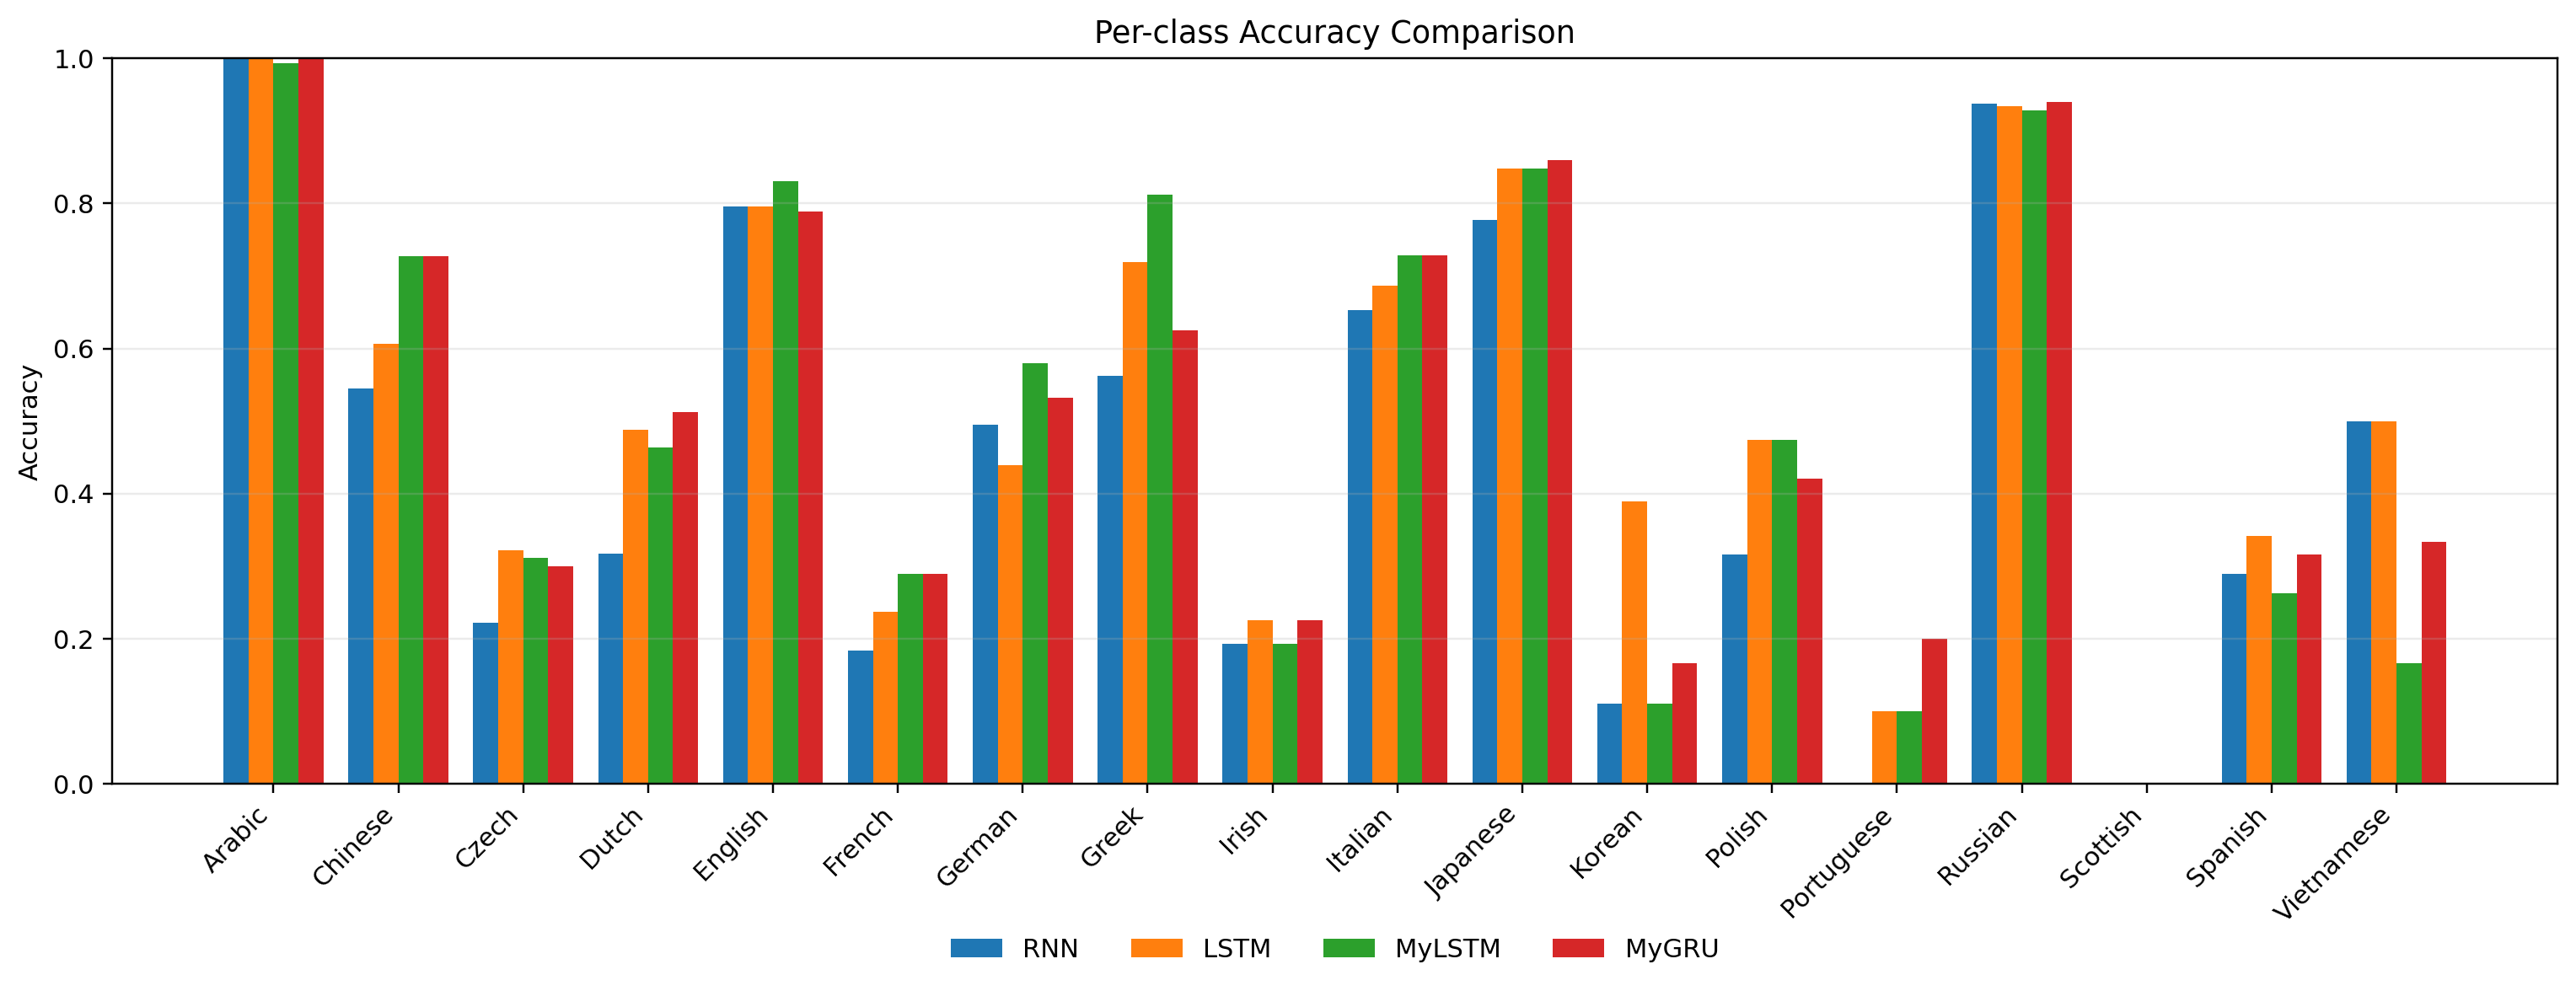
\includegraphics[width=\textwidth]{class_accuracy_compare.png}
    \caption{四种分类模型在测试集上的各类别准确率对比。}
    \label{fig:class_acc_compare}
\end{figure}

从图 \ref{fig:class_acc_compare} 可以看出，门控结构带来的优势并不是只体现在个别类别上，而是在多个语言类别上都有较稳定的提升。例如大样本类别 Russian、English、Japanese 的识别较为稳定，而小样本类别如 Scottish、Portuguese 则更容易受到数据不平衡影响。以 Scottish 为例，测试集中只有 15 个样本，而且与 English 在字符模式上较接近，因此多个模型都更容易将其误判为 English，这也从侧面说明总体准确率之外，类别级别分析同样重要。

\begin{table}[H]
\centering
\caption{RNN 与 LSTM 在不同名字长度区间上的测试集准确率对比}
\begin{tabular}{lcccc}
\toprule
Model & 1--5 & 6--8 & 9--12 & 13+ \\
\midrule
RNN & 0.6710 & 0.8076 & 0.8973 & 0.9286 \\
LSTM & \textbf{0.6942} & \textbf{0.8199} & \textbf{0.9093} & 0.9286 \\
\bottomrule
\end{tabular}
\label{tab:length_group}
\end{table}

表 \ref{tab:length_group} 表明，在 1--12 个字符区间内，LSTM 的准确率始终略高于 RNN，说明门控记忆机制在短到中等长度名字上具有稳定优势。对于 13+ 区间，两种模型的准确率相同，但该组仅包含 28 个样本，样本量过少，因此不宜据此对最长序列上的性能差异作出强结论。

\subsection{曲线图和预测矩阵图展示}
这一小节统一展示原始 RNN、个人实现的 \texttt{myLSTM} 以及手写 \texttt{myGRU} 在名字识别验证集上的训练曲线与预测矩阵图。

从图 \ref{fig:three_model_curves} 可以整体看出，三种模型的 train loss 都能够持续下降，但训练曲线和验证曲线都存在一定波动，说明在本实验设置下，batch size=128 对该任务而言仍然偏小，梯度估计中保留了较明显的随机性。因此，各模型在训练过程中并没有表现出非常平滑的收敛轨迹。与此同时，验证集曲线在达到较优位置后普遍进入平台期，部分模型的 val loss 还会在后期回升，说明名字识别任务中仍然存在一定程度的过拟合现象。因此，仅看最后一个 epoch 并不合适，本文统一以验证集最佳结果对应的 checkpoint 作为最终模型。

如表 \ref{tab:best_model_summary} 所示，手写 \texttt{myGRU} 的最佳验证准确率达到 83.46\%，是四个分类模型中验证集表现最好的模型，而手写 \texttt{myLSTM} 的测试集准确率达到 82.27\%，在测试集上表现最佳。对比三列曲线可以发现，带门控的 \texttt{myLSTM} 和 \texttt{myGRU} 在训练前期收敛更快，验证集准确率上升也更明显，而原始 RNN 更早进入饱和状态。

\begin{figure}[H]
    \centering
    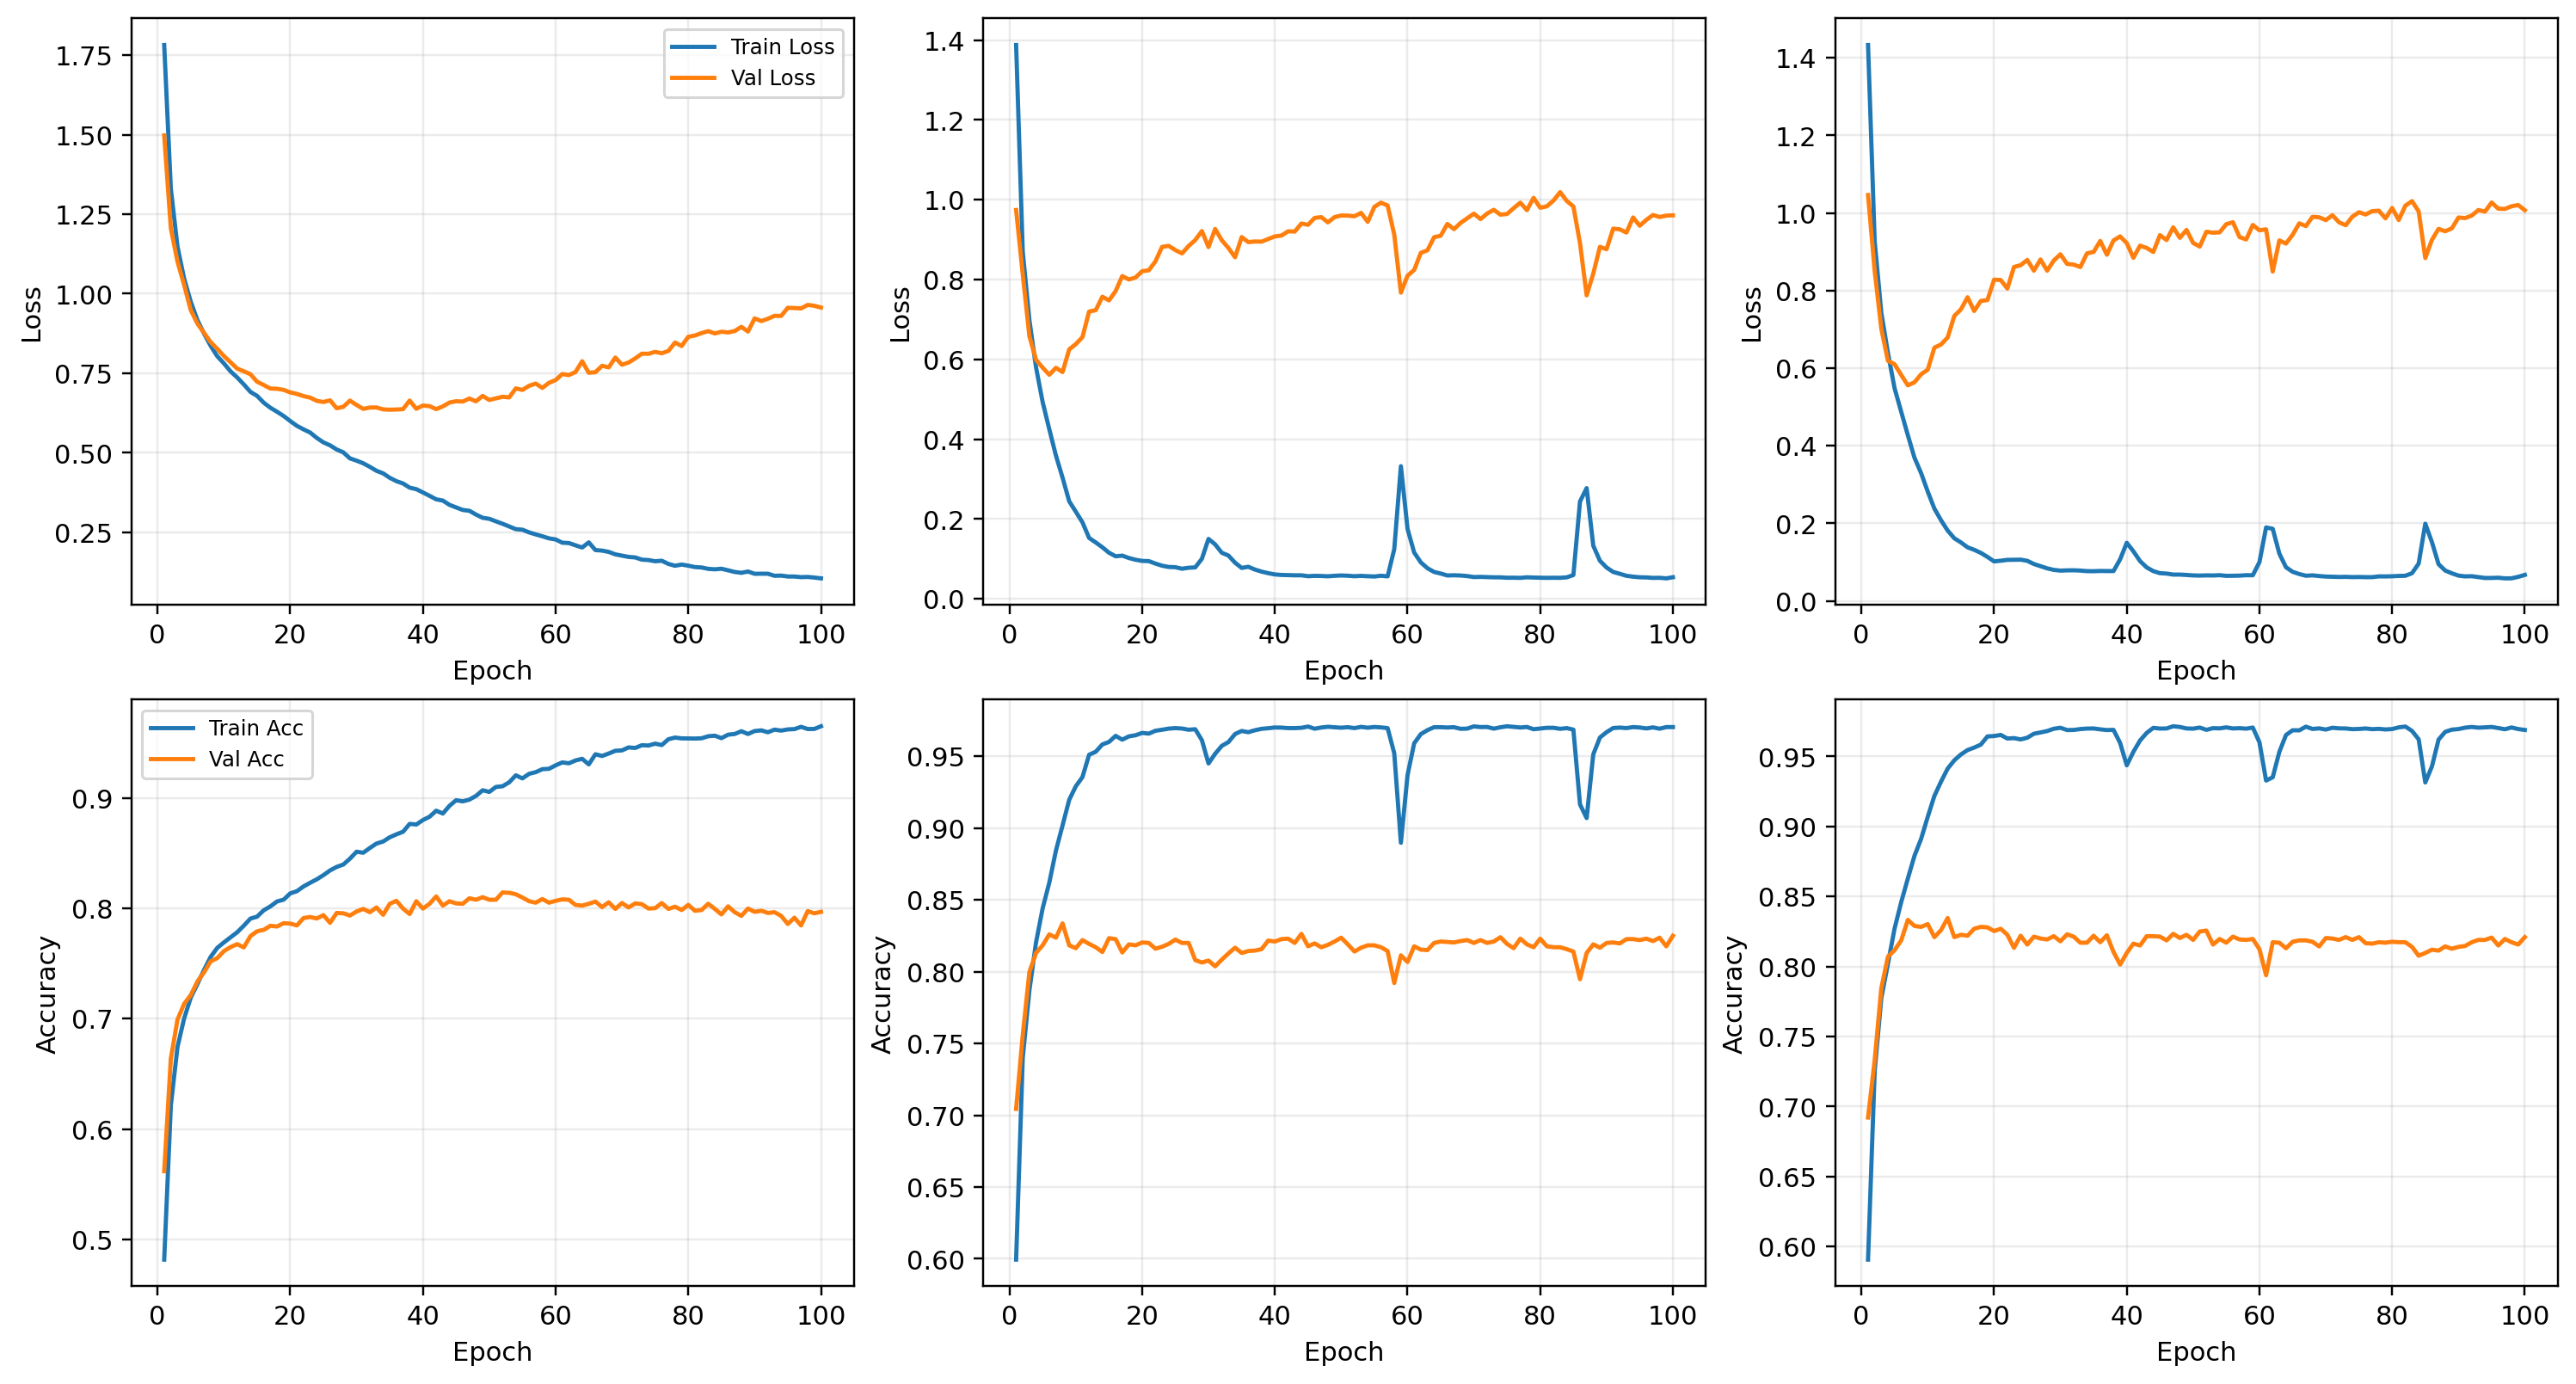
\includegraphics[width=\textwidth]{generated/rnn_mylstm_mygru_curves_grid.png}
    \caption{原始 RNN、手写 \texttt{myLSTM} 与手写 \texttt{myGRU} 在验证集上的训练/验证损失与准确率曲线对比。}
    \label{fig:three_model_curves}
\end{figure}

\begin{figure}[H]
    \centering
    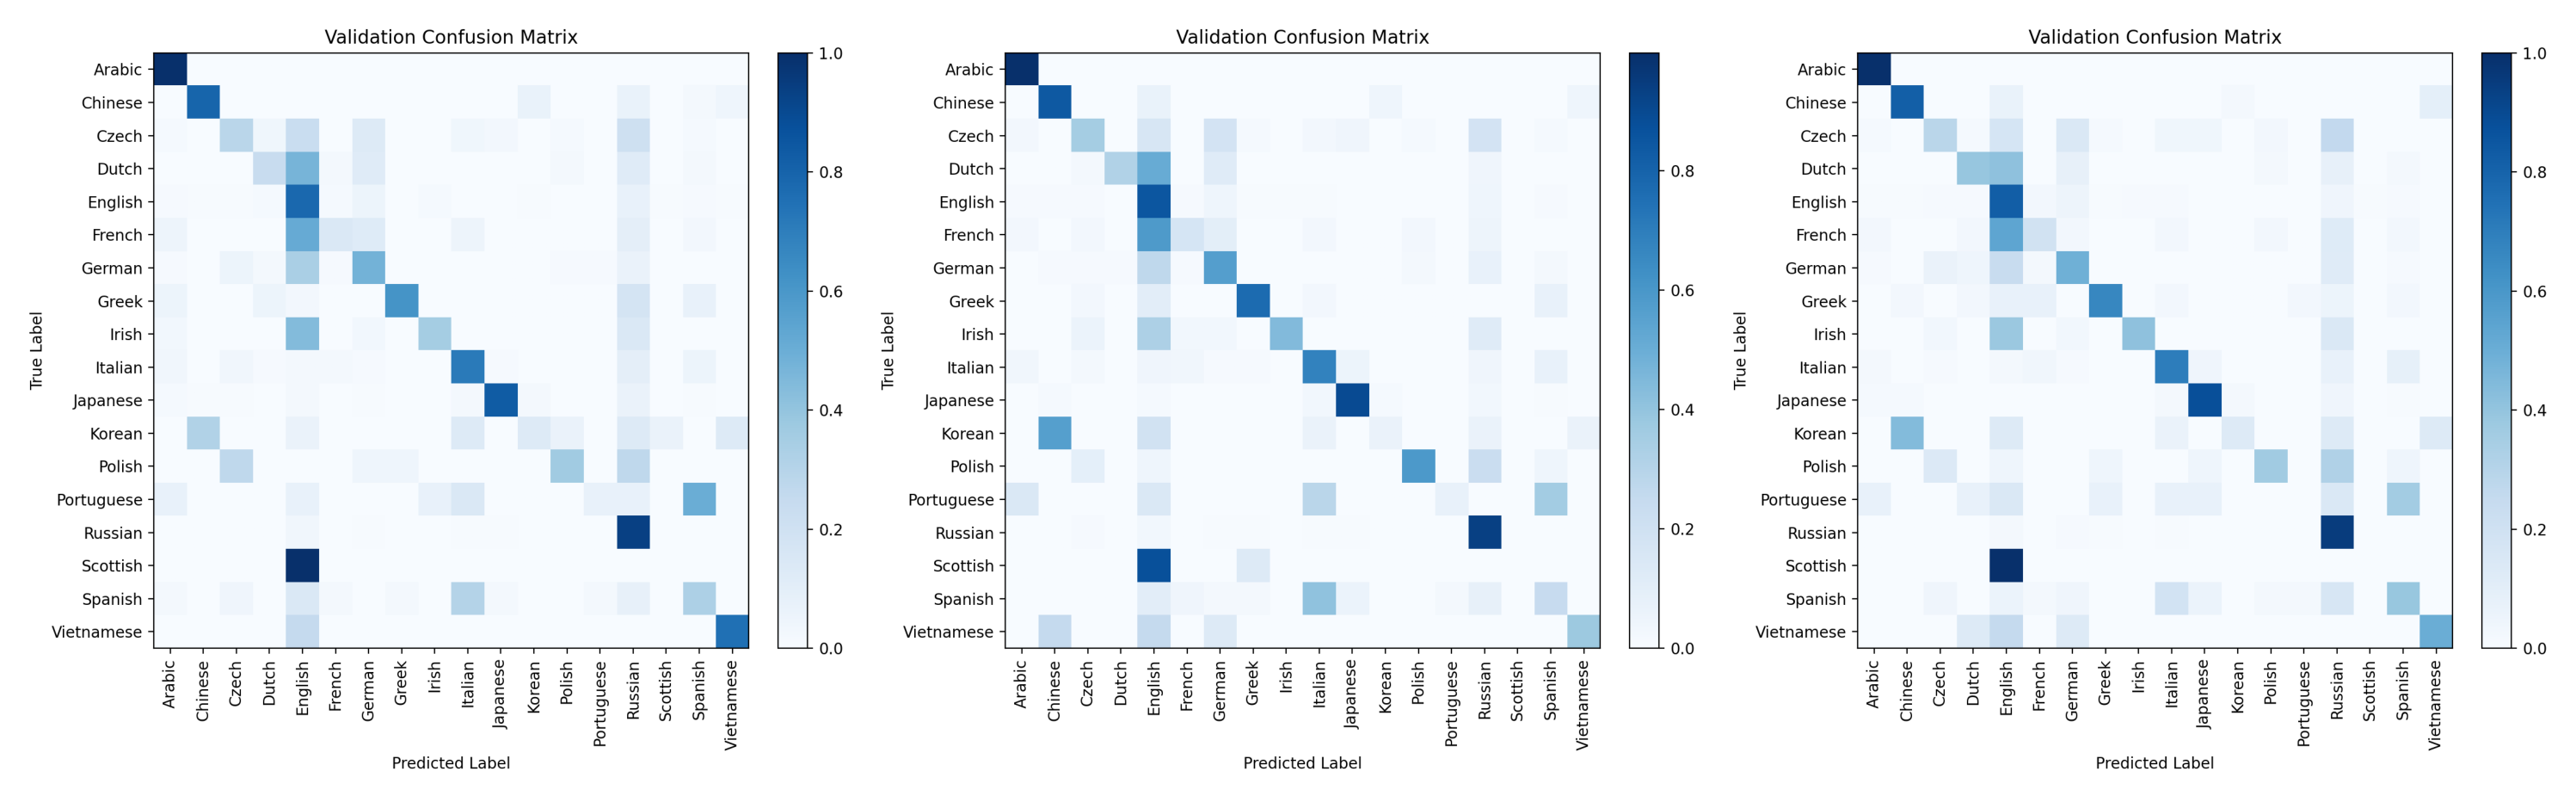
\includegraphics[width=\textwidth]{generated/rnn_mylstm_mygru_confusion_grid.png}
    \caption{原始 RNN、手写 \texttt{myLSTM} 与手写 \texttt{myGRU} 在验证集上的预测矩阵图对比。}
    \label{fig:three_model_confusion}
\end{figure}

从图 \ref{fig:three_model_confusion} 可以看到，三种模型的混淆矩阵整体形态其实较为接近：主对角线逐渐增强，但若干相近语言之间仍然持续存在混淆。这说明除了模型结构差异外，数据集本身的语言相似性也是影响识别结果的重要因素。例如若干拼写模式接近的语言即使在门控模型中也不容易完全分开。不过，与原始 RNN 相比，\texttt{myLSTM} 和 \texttt{myGRU} 的主对角线更集中，非对角元素略少，说明门控机制确实提高了模型对细粒度字符模式的利用能力，但并不能完全消除由语言本身相似性和类别不平衡带来的分类难点。

\subsection{内置 LSTM 与手写模型的补充对比}
除了手写 \texttt{myLSTM} 和 \texttt{myGRU} 之外，本文还训练了基于 \texttt{nn.LSTM} 的内置 LSTM。如表 \ref{tab:best_model_summary}所示，内置 LSTM、手写 \texttt{myLSTM} 和手写 \texttt{myGRU} 都明显优于原始 RNN，说明性能提升的关键是门控循环结构本身。

从实现角度看，\texttt{torch} 自带的内置 LSTM 经过了更充分的底层优化，因此在训练时间与推理时间方面更具优势（见表 \ref{tab:efficiency_summary}）；而手写 \texttt{myLSTM} 和 \texttt{myGRU} 的主要价值在于可以显式展示遗忘门、输入门、输出门或更新门、重置门的计算过程，更适合理解状态更新机制。

\subsection{梯度稳定性实验}
本文还对梯度范数变化进行了额外观察。实验中发现，在当前任务规模、学习率和隐藏层维度设置下，训练过程中的梯度峰值并不高，远低于此前设置的 5.0 裁剪阈值，因此在分类实验中关闭梯度裁剪后，模型训练并未出现明显发散。这个现象说明，在本实验的配置下，梯度裁剪并不是影响最终性能的关键因素；相比之下，循环结构本身是否具有门控记忆机制，对最终分类结果的影响更大。

\begin{figure}[H]
    \centering
    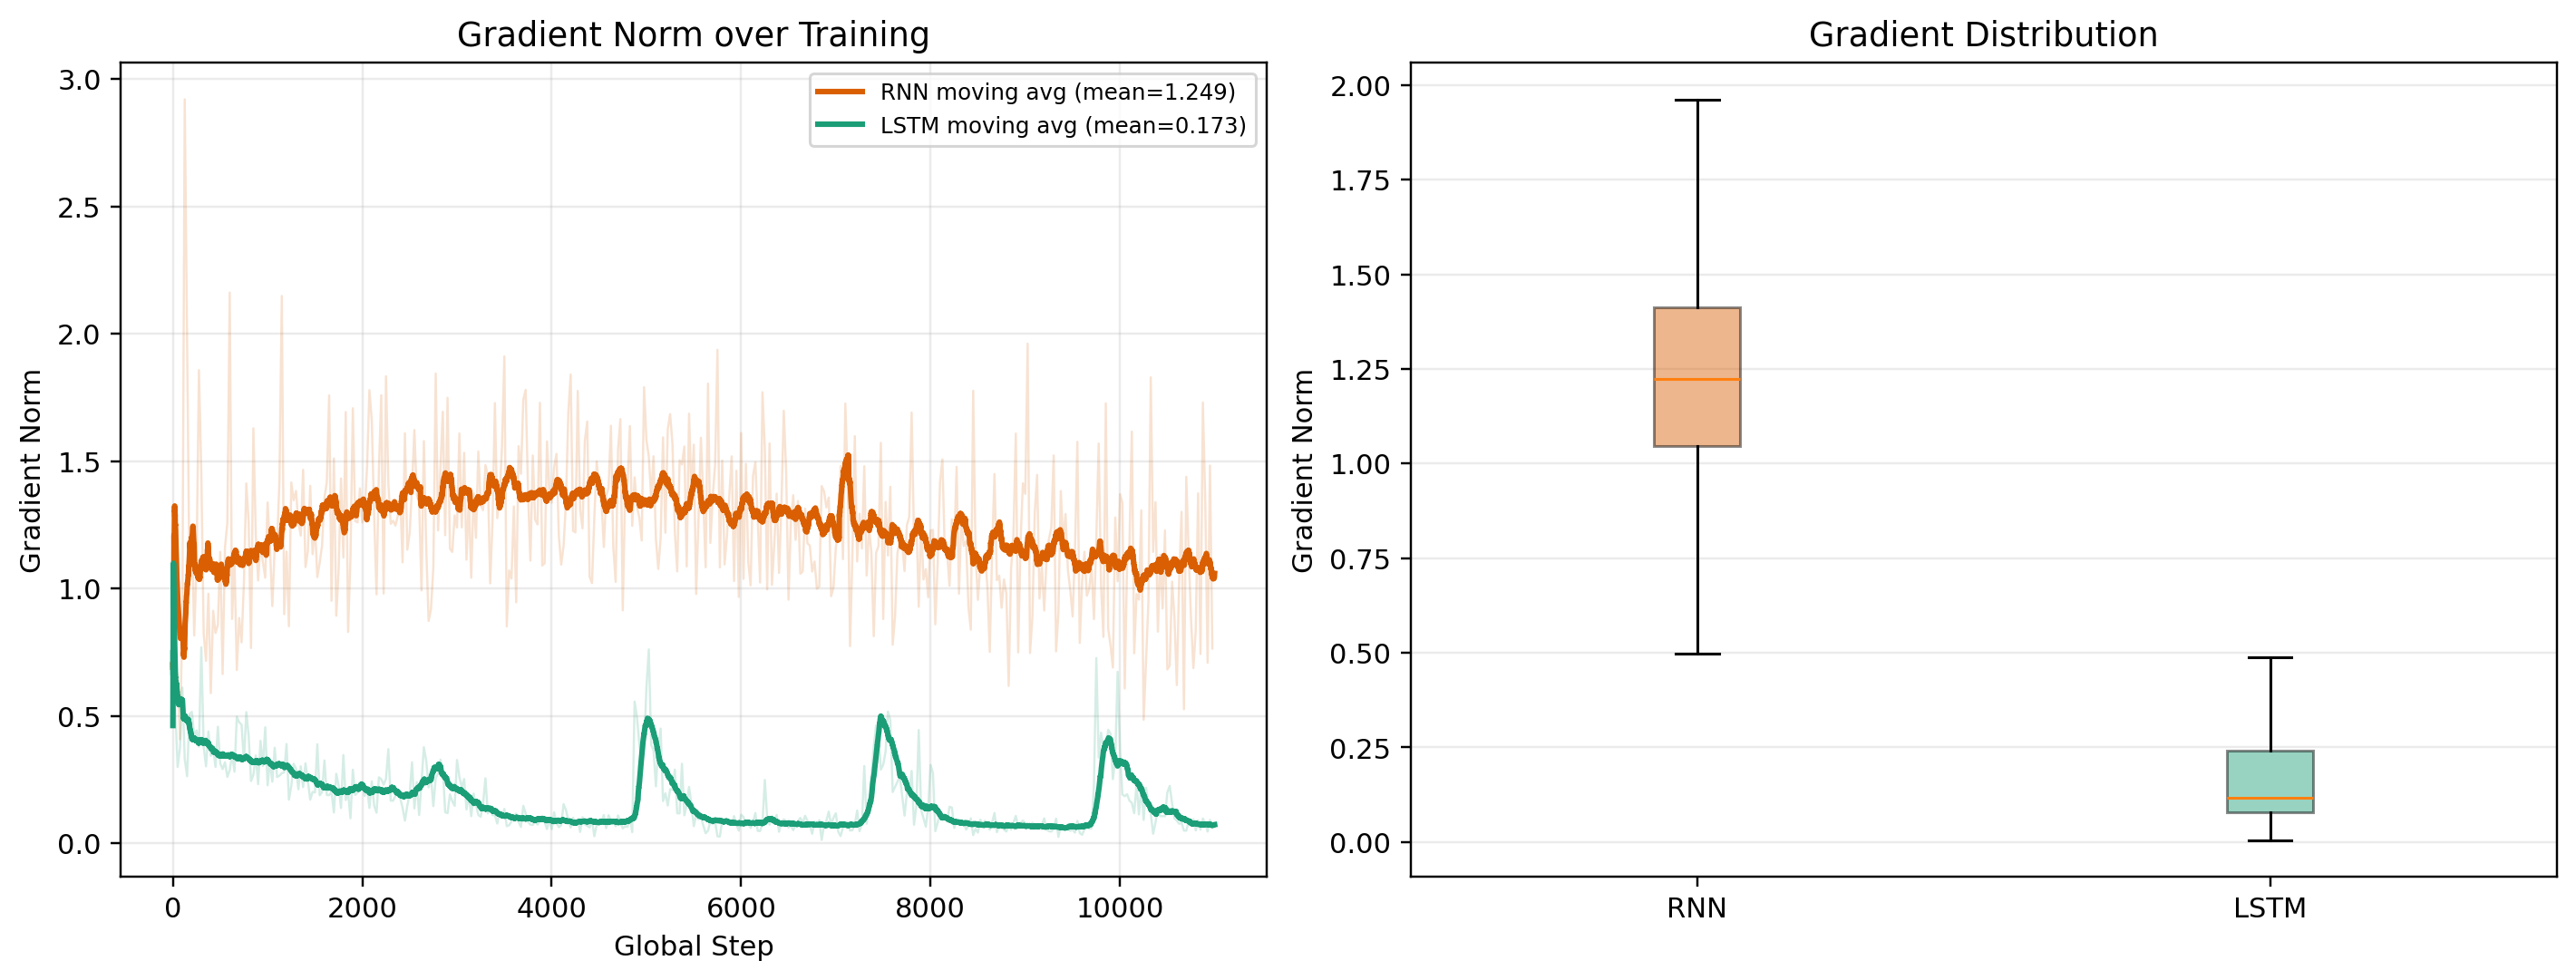
\includegraphics[width=\textwidth]{generated/rnn_lstm_gradient_compare.png}
    \caption{原始 RNN 与 LSTM 在训练过程中的梯度范数对比。左图为随训练步数变化的平滑梯度曲线，右图为梯度分布箱线图。}
    \label{fig:rnn_lstm_gradient}
\end{figure}

从图 \ref{fig:rnn_lstm_gradient} 可以看出，原始 RNN 的梯度整体明显大于 LSTM，且波动范围更宽。这并不意味着“梯度越大越好”，相反，它说明普通 RNN 在时间维度上的误差传播更不稳定。由于 RNN 在每个时间步都需要反复对隐藏状态进行非线性更新，梯度在反向传播过程中更容易出现放大和震荡；而 LSTM 通过 cell state 与门控机制对信息流进行调节，使梯度传播更加平稳、受控。因此，在本实验中，LSTM 不仅取得了更高的验证集和测试集准确率，其训练过程也表现出更好的优化稳定性。这一现象与原始 LSTM 论文中关于“LSTM 更适合处理长期依赖和稳定传播误差信号”的观点是一致的\cite{hochreiter1997lstm}。

\subsection{名字生成实验}
\subsubsection{生成任务设置}
为了进一步比较不同循环网络在字符级序列建模中的差异，本文在名字识别任务之外扩展了条件名字生成实验。生成模型包括 \texttt{rnn\_gen}、\texttt{lstm\_gen} 和 \texttt{gru\_gen} 三种结构（由于手动实现版本训练太久，这里都是用内置版本进行实验），训练目标为：在给定语言类别和当前字符的条件下，预测下一个字符，直到生成 EOS 结束标记。本实验的评判标准比较主观，用判别器计算损失时间花销难以接受，这里选取trainloss最小的checkpoint为最佳。然后各模型从最佳 checkpoint 中重新采样，在全部 18 个类别上每类生成 100 个名字。

\subsubsection{类别一致性评估}
单纯观察生成名字是否“像名字”仍然偏主观，因此本文引入了类别一致性评估：利用已经训练好的最佳 LSTM 分类器作为判别器，将生成名字重新送入分类器，检查它是否还能被判成目标语言类别。若条件类别和分类器预测类别一致，则记为一次命中；对所有生成样本统计命中比例，就得到该生成模型的 category fidelity。

\begin{table}[H]
\centering
\caption{三种生成模型的整体类别一致性对比}
\begin{tabular}{lccc}
\toprule
Model & Best LR & Overall Fidelity & Avg Name Length \\
\midrule
RNN Generation & 0.001 & 0.4972 & 5.5150 \\
LSTM Generation & 0.005 & \textbf{0.7161} & 6.5261 \\
GRU Generation & 0.005 & 0.6761 & 6.2617 \\
\bottomrule
\end{tabular}
\label{tab:generation_fidelity}
\end{table}

表 \ref{tab:generation_fidelity} 表明，在名字生成任务上，LSTM generation 的整体类别一致性最高，GRU generation 次之，而 RNN generation 明显更低。这说明门控结构不仅有助于分类任务中的长期信息保留，也有助于生成任务中维持更稳定的语言风格。

% \begin{figure}[H]
%     \centering
%     \includegraphics[width=0.72\textwidth]{../outputs/generation/fidelity_reports/baseline_lstm_judge/overall_fidelity.png}
%     \caption{三种生成模型的整体类别一致性对比。}
%     \label{fig:overall_fidelity}
% \end{figure}

\begin{figure}[H]
    \centering
    \includegraphics[width=\textwidth]{../outputs/generation/fidelity_reports/baseline_lstm_judge/category_fidelity.png}
    \caption{不同语言类别上的生成类别一致性对比。}
    \label{fig:category_fidelity}
\end{figure}

从图 \ref{fig:category_fidelity} 可以进一步看到，不同模型的生成质量差异并不是均匀分布的。对于 Arabic、English、Russian、Japanese 等模式较强的大类，三种生成模型都相对更容易保持类别风格；而 Portuguese、Scottish、Irish、French 等类别更容易发生风格偏移，其中 RNN generation 的偏移最明显。例如在本实验中，RNN generation 在 Portuguese 和 Scottish 上的 fidelity 接近 0，而 LSTM generation 和 GRU generation 虽然也较难，但仍然明显更高。这说明门控结构在生成复杂或小样本语言风格时依然具有优势。

此外，类别一致性评估还有一个重要意义：它不仅评估“生成结果像不像名字”，更评估“生成结果像不像目标语言的名字”。因此，这一指标比单纯展示若干生成样例更适合作为生成质量的量化标准。结合识别任务的结果可以看出，LSTM/GRU 相比原始 RNN 的优势并非只体现在分类上，也同样体现在生成过程中对目标语言风格的保持能力上。

\section{为什么 LSTM 网络的性能优于 RNN 网络}
普通 RNN 在每个时间步只维护一个隐藏状态，前一时刻的所有信息都必须压缩在同一个向量中继续往后传递。当序列稍长时，早期字符信息在多次非线性变换后更容易逐渐衰减，因此模型往往难以稳定保留前缀、后缀和局部字符模式之间的长距离依赖关系。名字识别任务虽然序列不算特别长，但语言风格往往同时体现在前缀、中缀和后缀上，因此这种长期信息保留能力依然非常重要。

原始 LSTM 论文指出，普通循环网络在长时滞任务上会受到梯度消失和梯度爆炸问题的影响，而 LSTM 的设计目标正是通过更稳定的误差传播路径来缓解这一问题\cite{hochreiter1997lstm}。论文中提出的核心思想是：在循环结构中引入能够长期保存信息的 memory cell，并通过门控机制控制信息写入、保留和输出，从而使网络能够跨更长的时间范围学习有效依赖关系\cite{hochreiter1997lstm}。具体到结构上，LSTM 引入了 cell state 和记忆门控机制。遗忘门决定旧记忆保留多少，输入门决定当前时刻写入多少新信息，输出门再控制当前隐藏状态对外暴露多少内容。这样一来，模型不需要像原始 RNN 那样把所有信息都硬压缩到一个不断重复更新的隐藏状态里，而是能够更有选择地保留有用字符模式，抑制无关扰动。从结构上看，这种设计正对应了原论文强调的“更稳定地保留长期信息”的目标\cite{hochreiter1997lstm}。

从本实验结果来看，这种理论优势在分类和生成两类任务中都得到了体现。首先，在分类任务中，LSTM 和手写 \texttt{myLSTM} 的最佳验证准确率与测试准确率都高于原始 RNN，验证集预测矩阵图的主对角线也更集中，说明模型对相近语言之间的区分能力更强。其次，长度分组实验只能说明 LSTM 在大多数长度区间上的表现更稳定，但由于数据集分布和样本规模的限制，它并不足以单独证明“LSTM 更适合更长序列”。而在生成任务中，LSTM 生成的名字平均长度更长，判别稳定性也更好，可以在一定程度上补充说明其序列建模优势；此外，LSTM generation 的整体类别一致性明显高于 RNN generation，这说明带门控的循环结构不仅在分类时更容易保留有效字符信息，在生成时也更能保持目标语言风格的一致性。

需要指出的是，LSTM 的参数量高于原始 RNN，更大的模型容量可能对性能提升有一定帮助；但结合内置 LSTM、手写 \texttt{myLSTM} 和手写 \texttt{myGRU} 的结果可以看出，性能改善并不能简单归因于参数量增加，更关键的原因仍在于门控循环结构对长期信息保留和状态更新方式的改进。因此，参数量可以视为影响因素之一，但不是本文中 LSTM 优于 RNN 的主要解释。进一步而言，后续还可以通过构造更深或更宽的 RNN（深度循环神经网络），使其参数规模尽量与 LSTM 对齐，从而更严格地区分“参数量增加”与“门控结构改进”对性能提升的贡献。受本文篇幅和实验范围限制，这一部分暂不展开。

综合来看，LSTM 优于 RNN 的根本原因并不只是“参数更多”，而是它的门控机制和细胞状态能够更稳定地保存长期信息，使模型在字符级序列分类和生成中都更容易学到真正有判别力的语言模式。

此外，由于本文的名字识别与名字生成任务都属于较短字符序列任务，因此它们并不能像原始 LSTM 论文中的人工长时滞实验那样，直接体现 LSTM 在极长距离依赖建模上的优势。长度分组实验只能说明 LSTM 在当前大多数名字长度区间上的表现更稳定，而不能据此直接推广到“更长文本任务”。同样，生成任务中的平均生成长度也只能提供有限线索。相比之下，更有说服力的证据来自分类准确率、混淆矩阵、梯度稳定性以及 category fidelity：这些结果共同说明，LSTM 在当前任务上更能稳定保留和利用跨时间步的有效信息。因而，这里更为谨慎的结论是：LSTM 在字符级序列建模中表现出更强的长期依赖建模能力和更高的训练稳定性，而其在真正长文本或长时滞任务上的优势，还需要通过实验进一步验证。

\section{实验结论}
本文围绕字符级名字识别和条件名字生成两个任务，对原始 RNN、内置 LSTM、手写 \texttt{myLSTM} 和手写 \texttt{myGRU} 进行了实现和比较。实验结果比较清楚地表明，带门控的循环结构整体上都优于原始 RNN：在识别任务中，手写 \texttt{myLSTM} 的测试集准确率最高，手写 \texttt{myGRU} 的验证集准确率最高，而内置 LSTM 在训练和推理效率上更有优势。也就是说，在当前名字分类任务上，门控循环结构在精度和稳定性上都更占优。

结合验证集曲线、预测矩阵图、梯度稳定性分析以及生成任务中的类别一致性结果可以看出，LSTM 优于原始 RNN 的主要原因并不只是参数更多，而在于门控机制和 cell state 让信息保留与状态更新更加稳定。相比之下，原始 RNN 虽然结构简单、参数量小，但在字符级序列中更容易受到信息衰减和训练波动的影响，因此在分类和生成两类任务上都表现出更明显的局限。手写 \texttt{myLSTM} 和 \texttt{myGRU} 的结果也说明，本文不仅调用了框架内置模块，也真正实现了门控循环网络的核心状态更新过程。

当然，本文使用的两个任务都属于较短字符序列任务，因此这些结果更多说明的是门控结构在短序列建模中的有效性，而不能完全替代原始 LSTM 论文里针对长时滞依赖的控制实验。另外，数据集本身还存在类别不平衡问题，一些小样本语言类别仍然比较难识别。总体来看，本文的实验支持这样一个结论：在当前字符级序列建模场景下，LSTM 和 GRU 相比原始 RNN 更稳定，也更容易取得更好的综合表现；至于它们在更长序列任务上的优势，还需要通过更长文本和更可控的实验进一步验证。

\newpage
\appendix
\section{代码目录说明}
为便于提交与查阅，本文将实验二的核心代码单独整理在 \texttt{lab2/code/} 目录下。该目录只保留训练入口、模型实现、评估脚本和结果生成脚本，不包含 \texttt{outputs/}、\texttt{docs/}、\texttt{old/} 等实验结果与参考材料。

如果希望先了解整体实验流程，建议优先查看：
\begin{itemize}
    \item \texttt{code/train.py}：名字识别任务训练入口；
    \item \texttt{code/train\_generation.py}：条件名字生成任务训练入口；
    \item \texttt{code/sweep\_lr.py}：分类任务学习率扫描；
    \item \texttt{code/evaluate\_generation\_fidelity.py}：生成任务类别一致性评估。
\end{itemize}

如果重点查看模型实现，建议从
\begin{itemize}
    \item \texttt{code/src/models/registry.py}
\end{itemize}
开始。该文件负责注册分类模型，便于跳转到具体实现。对应的核心模型文件为：
\begin{itemize}
    \item 原始 RNN：\texttt{code/src/models/rnn.py}
    \item 内置 LSTM：\texttt{code/src/models/lstm.py}
    \item 手写 myLSTM：\texttt{code/src/models/myLSTM.py}
    \item 手写 myGRU：\texttt{code/src/models/myGRU.py}
    \item 生成模型：\texttt{code/src/models/name\_generator.py}
\end{itemize}

另外，所有运行脚本已经统一整理到 \texttt{code/scripts/} 目录下。例如分类任务批量运行脚本为 \texttt{code/scripts/run.sh}，生成任务学习率扫描脚本为 \texttt{code/scripts/sweep\_lr\_generation.sh}。其余支撑模块中，\texttt{code/src/data.py} 与 \texttt{code/src/generation\_data.py} 负责数据组织，\texttt{code/src/engine.py} 与 \texttt{code/src/generation\_engine.py} 负责训练与评估主循环，\texttt{code/src/utils/} 下则包含结果写出、作图、性能统计等工具函数。

\bibliographystyle{plain}
\bibliography{reference}

\end{document}
